\documentclass{article}
\usepackage{tikz}

\begin{document}
	\begin{center}
		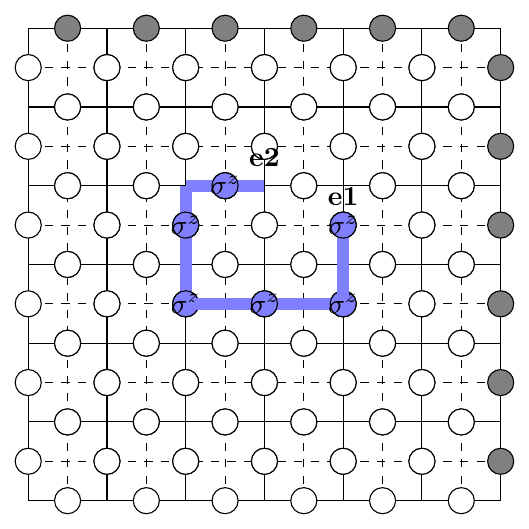
\begin{tikzpicture}
			% Draw dashed lines
			\foreach \i in {-3,-2.5,...,3}
			{
				\draw[dashed] (\i,-3) -- (\i,3);
			}
			\foreach \j in {-3,-2.5,...,3}
			{
				\draw[dashed] (-3,\j) -- (3,\j);
			}
			
			
			% Draw solid grid and nodes with circles in the middle of each side
			\draw[step=1cm] (-3,-3) grid (3,3);
			\foreach \i in {-2.5,...,2.5}
			{
				\foreach \j in {-2.5,...,2.5}
				{
					\begin{scope}[transform canvas={xshift=\i cm,yshift=\j cm}]
						\node[right,xshift=0.2cm,yshift=0.4cm] {};
						% Convert \j and \i to integers
						\pgfmathtruncatemacro{\intj}{\j}
						\pgfmathtruncatemacro{\inti}{\i}
						
						% Draw circles at the midpoints of each side
						\ifnum\intj=2
						\draw node[draw,circle,fill=gray] at (0,0.5) {};
						\else
						\draw node[draw,circle,fill=white] at (0,0.5) {};
						\fi
						
						\ifnum\inti=2
						\draw node[draw,circle,fill=gray] at (0.5,0) {};
						\else
						\draw node[draw,circle,fill=white] at (0.5,0) {};
						\fi
						
						\draw node[draw,circle,fill=white] at (0,-0.5) {};
						\draw node[draw,circle,fill=white] at (-0.5,0) {};
					\end{scope}
				}
			}
		
			
			
			
			\foreach \j in {1,...,1}
			{
				
				\draw[blue!50, line width=1.5mm] (-1, \j) -- (-0.5, \j);
				\draw node[label=north:\textbf{e2}] at (0,\j) {};
				\draw[blue!50, line width=1.5mm] (-0.5, \j) -- (0, \j);
				
				\node[draw, circle, fill=blue!50,label=center:\textbf{$\sigma^z$}] at (-0.5,1) {};
				
			}
			
			\foreach \i in {-1,...,-1}
			{
				
				\draw[blue!50, line width=1.5mm] (\i,1) -- (\i,-0.5);
				%\draw node[label=north:\textbf{e1}] at (\i,0) {};
				%\draw[blue!50, line width=1.5mm] (\i,0) -- (\i,0);
				
				\node[draw, circle, fill=blue!50,,label=center:\textbf{$\sigma^z$}] at (-1,0.5) {};
				\node[draw, circle, fill=blue!50,,label=center:\textbf{$\sigma^z$}] at (-1,-0.5) {};
				
			}
			
			\foreach \j in {-0.5,...,-0.5}
			{
				
				\draw[blue!50, line width=1.5mm] (-0.9, \j) -- (1, \j);
				
				
				\node[draw, circle, fill=blue!50,label=center:\textbf{$\sigma^z$}] at (0,-0.5) {};
				\node[draw, circle, fill=blue!50,label=center:\textbf{$\sigma^z$}] at (1,-0.5) {};
				
			}
			
			\foreach \i in {1,...,1}
			{
				
				\draw[blue!50, line width=1.5mm] (\i,-0.4) -- (\i,0.5);
				\draw node[label=north:\textbf{e1}] at (\i,0.5) {};
				%\draw[blue!50, line width=1.5mm] (\i,0) -- (\i,0);
				
				\node[draw, circle, fill=blue!50,,label=center:\textbf{$\sigma^z$}] at (1,0.5) {};
				
			}
			
			
			
		\end{tikzpicture}
	\end{center}
	
\end{document}
